\documentclass[twocolumn,10pt,a4j]{jsarticle}
\usepackage{kougai}
\usepackage{dcolumn}


\title{OffscreenCanvasを用いたシミュレータ教材の軽量化}
\author{1532040 岡本 悠祐  指導教員 須田 宇宙 准教授}
\date{}
 
\begin{document}
\maketitle
\section{背景}
シミュレータ教材は不可視現象を可視化する教材である.そのため,イメージが困難な事象への理解促進を促す手法として有用である.
e-Learningの普及に伴いシミュレータ教材の活躍の場が増加し,様々な分野に対応したシミュレータ教材と効率的な開発手法が必要とされている.

磁場や音場などの波形を可視化するシミュレータにおいてFTDT(Finite-difference time-domain )法が広く用いられているが演算回数が多いことから処理速度は決して速くない.

本研究室では昨年,FTDT法を用いたシミュレータ教材にGPUを適用しCPUとの処理速度を比較する研究を行った.その結果,大幅な処理速度向上が得られたが,ソースコードの変更箇所が多く,
複雑なため容易に実装できないという問題点が浮上した.

その問題点はJavaScriptでWorkerを活用し,描画を行うOffscreenCanvasを利用することで緩和されると考える.

本研究ではOffscreenCanvasを利用したFTDT法を用いたシミュレータ教材の制作を行い,ソフトウェアの生産性と処理速度を昨年制作したシミュレータ教材と比較することで,有用性の検証を行うことを目的とする.

\begin{comment}

\section{WebWorkerとOffscreenCanvas}
\subsection{WebWorker}
WebWorkerはJavaScriptでマルチスレッド処理を可能にするAPIである.Workerを利用するには処理ごとにファイルを分ける.
また,Worker上で描画を行うことができないため描画処理を行いたい場合は,Workerを定義するメインのスレッドに対して描画処理を渡す必要がある.

\subsection{OffscreenCanvas}
OffscreenCanvasはWebWorkerを利用してWorker上で描画処理を可能にするAPIである.

事前にCanvasタグをHTMLないしJavaScriptで生成し,Workerに処理を譲渡,描画まで行うため,Workerより必要な処理が少なく手軽に実装できる.

\end{comment}

\section{制作したシミュレータ教材}
本研究ではOffscreenCanvasを利用したシミュレータ教材の有用性の検証を行う.プログラムには昨年本学卒業論文である「GPU利用によるシミュレータ教材の演算速度」を拡張し,処理速度とソースコードの比較を行う.

図\ref{fig:one}は本研究で制作した複数の音源から発生する音場を可視化したシミュレータである.本研究では図\ref{fig:two}のようにキャンバスを左右に分けることにより,負荷を分散させた.


\begin{figure}[htbp]
 \begin{minipage}{0.49\hsize}
  \begin{center}
   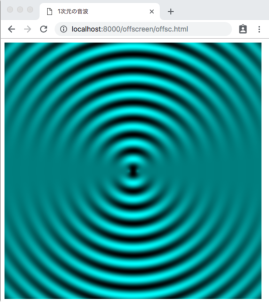
\includegraphics[width=30mm]{sim.pdf}
  \end{center}
  \caption{制作したシミュレータ}
  \label{fig:one}
 \end{minipage}
 \begin{minipage}{0.49\hsize}
  \begin{center}
  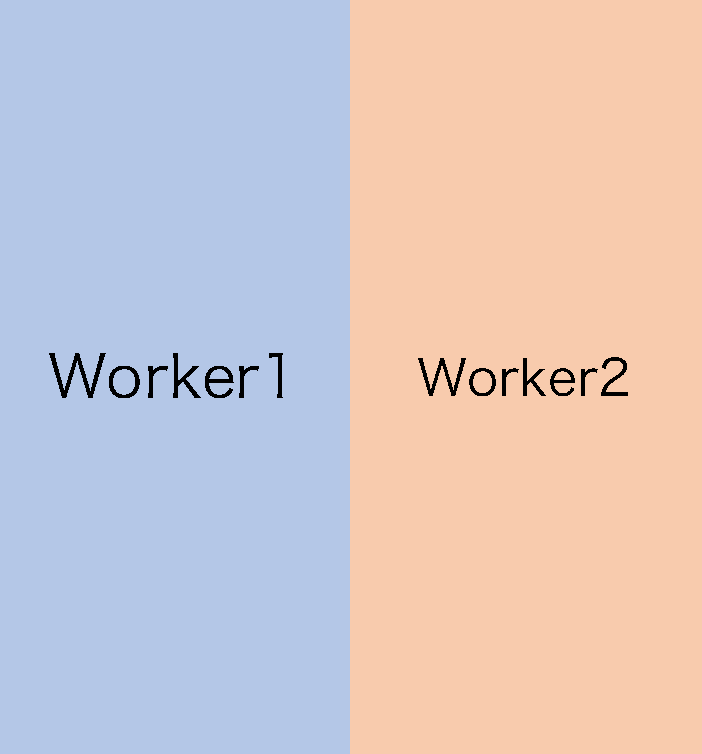
\includegraphics[width=30mm]{wake.pdf}
  \end{center}
  \caption{キャンバス分割イメージ}
  \label{fig:two}
 \end{minipage}
\end{figure}

\section{検証方法}
昨年のシミュレータと演算速度を比較,変更箇所を比較することでOffscreenCanvasの実用性の検証を行う.
 
1,000回計算する時間を計測,10,000回まで行った.比較に昨年のプログラム2つとOffscreenCanvas,Workerを利用した4つを用いた.

計測に使用したPCのスペックを表 \ref{tab:tab1}に示す.

\begin{table} [h]
\centering
\caption{使用したMacのスペック}
	\begin{tabular} {| c | c |} \hline
	OS & macOS HIigh Sierra \\ \hline
	メモリ & 32GB \\ \hline
	CPU & 3.2GHz Intel Core i5 \\ \hline
	GPU & NVIDIA GeForce GT 775M 1024MB\\ \hline
	\end{tabular} 
	\label{tab:tab1}
\end{table}



\section{検証結果}
昨年制作されたシミュレータ教材ではCPUとGPUの処理速度の比較を行った.ここでは昨年に制作され,CPUで動作させた方をCPU,GPUで動作させた方をGPUと呼ぶ.CPUの処理速度を基準とし,各処理速度を式\ref{eq:eq1}に当てはめて求めた.

キャンバスを分割したWebWorkerとOffscreenCanvasは処理速度が遅い方を参照する.その結果を表\ref{tab:tab2}に記した.
\begin{equation}
 処理効率 = \frac { 各手法10,000回の処理速度 [ms]} { 基準10,000回の処理速度[ms] } 
\label{eq:eq1}
\end{equation}


\begin{table} [h]
\centering
\caption{各種法の処理速度比較}
	\begin{tabular} {| c | l D{.}{.}{8} |} \hline
	GPU & 1: & 0.810988 \\ \hline
	OffscreenCanvas & 1: & 0.80789763 \\ \hline
	WebWorker & 1: & 0.795556697 \\ \hline
	\end{tabular} 
	\label{tab:tab2}
\end{table}

OffscreenCnavasの変更箇所は分割したキャンバスの範囲指定と,キャンバスの生成元であるHTMLのキャンバスを増やすだけで,ソースコードの変更点はほとんどなかった.

Workerのみと違いworkerを宣言するメインではデータのデータの引き渡しがないだけでなく,左右のキャンバスを整合性をとる必要がないことからOffscreenCanvasはWorkerより実装が容易である.

\section{終わりに}
本研究ではOffscreenCanvasのFTDT法を用いたシミュレータへの有用性を検証した.
OffscreenCanvasはまだ出たばかりの技術のため,最適化されていない可能性があり,今後のさらなる改良と,知識の共有が必要である.
\begin{thebibliography}{99}

	\bibitem{book}土井 淳:``ソフトウェアの生産性に着目したGPUプログラミングの方法論に関する研究動向'',電子情報通信学会誌,Vol.101,pp1219-1223(2018)
\end{thebibliography}
\end{document}
